\documentclass[letterpaper]{article} % DO NOT CHANGE THIS
\usepackage[submission]{aaai2027}  % DO NOT CHANGE THIS
\usepackage[hyphens]{url}  % DO NOT CHANGE THIS
\usepackage{graphicx} % DO NOT CHANGE THIS
\urlstyle{rm} % DO NOT CHANGE THIS
\def\UrlFont{\rm}  % DO NOT CHANGE THIS
\usepackage{natbib}  % DO NOT CHANGE THIS AND DO NOT ADD ANY OPTIONS TO IT
\usepackage{caption} % DO NOT CHANGE THIS AND DO NOT ADD ANY OPTIONS TO IT
\frenchspacing  % DO NOT CHANGE THIS
\usepackage{algorithm}
\usepackage{algorithmic}
\usepackage{booktabs}
\usepackage{amsmath}
\usepackage{amssymb}

\pdfinfo{
/TemplateVersion (2027.1)
}

\setcounter{secnumdepth}{0}

\title{Affective Intelligence: Steering LLM Responses Through\\Affect Control Theory and Representation Engineering}
\author{
    Anonymous Submission
}
\affiliations{
    Anonymous Institution
}

\begin{document}

\maketitle

\begin{abstract}
Large language models (LLMs) generate responses without explicit models of socio-emotional dynamics, leading to behaviours such as sycophancy---excessive agreeableness that undermines trust and utility. We propose a novel framework that combines \textit{Affect Control Theory} (ACT), a mathematical sociological model of affective interaction, with \textit{Representation Engineering} (RepE), a technique for reading and steering high-level properties in neural network hidden states. Our system (1) reads the affective meaning of a user's message from the model's internal representations along three universal dimensions---Evaluation, Potency, and Activity, (2) uses ACT's impression-formation equations to compute the socially optimal affective response given the interactants' social identities, and (3) steers the model's generation by injecting calibrated activation vectors---all at inference time without weight modification. We evaluate four conditions---unsteered, prompt engineering only, RepE steering only, and a hybrid combining both---across 1,300 interaction scenarios spanning 13 identity pairs and 10 scenario categories, evaluated on two architectures (Llama-3.1-8B and Ministral-8B). Automated metrics show that the hybrid method achieves the lowest overall distance to ACT-predicted targets (e.g., 0.795 vs.\ 0.905 unsteered on Llama-3.1-8B, $p < 0.001$). A human evaluation study ($N = 48$, 672 ratings per condition) reveals significant differences across conditions for all three quality dimensions---appropriateness ($H = 70.92$, $p < 10^{-15}$), naturalness ($H = 73.47$, $p < 10^{-15}$), and non-sycophancy ($H = 127.85$, $p < 10^{-27}$)---with RepE-steered responses rated most non-sycophantic (mean~5.76/7) while maintaining naturalness comparable to unsteered baselines. These results demonstrate that sociological theory can provide principled steering targets for representation engineering, offering a training-free approach to socially grounded affective control of LLMs.
\end{abstract}

\section{Introduction}

Large language models (LLMs) have become integral to human-facing applications ranging from customer support to mental health counselling. However, a persistent concern is \textit{sycophancy}---the tendency of instruction-tuned models to produce excessively agreeable, flattering, or validating responses \citep{sharma2024understanding, perez2023discovering}. Sycophantic behaviour emerges as a side-effect of reinforcement learning from human feedback (RLHF), which rewards responses that users rate highly, creating incentives for models to agree rather than inform \citep{ouyang2022training, christiano2017deep}. This undermines user trust \citep{sun2025friendly} and is particularly problematic in contexts where honest, role-appropriate feedback is essential---a doctor should not flatter a patient, and a boss should not defer to a subordinate.

The core challenge is that LLMs lack an explicit model of the \textit{socio-emotional dynamics} of a conversation. They do not reason about how a response will be perceived relative to the social roles of the interactants, nor do they have a mechanism for selecting the affectively appropriate response given the situation.

We address this gap by combining two complementary frameworks. \textbf{Affect Control Theory} (ACT; \citealt{heise2007expressive}) is a mathematical sociological model that predicts how people select behaviours to confirm culturally-shared affective meanings. It operates over three universal dimensions---Evaluation (good--bad), Potency (powerful--weak), and Activity (active--passive)---and provides closed-form equations for computing the optimal affective response given the social identities and the preceding interaction event. \textbf{Representation Engineering} (RepE; \citealt{zou2023representation}) enables reading and controlling high-level cognitive properties in LLM hidden states using linear probes and activation perturbation, without modifying model weights.

Our contributions are:
\begin{enumerate}
    \item A novel pipeline that \textit{reads} affective meaning from LLM representations, \textit{computes} socially optimal targets using ACT, and \textit{steers} generation via activation addition---all at inference time.
    \item An empirical comparison of four steering conditions across 1,300 scenarios, demonstrating that hybrid (prompt + RepE) steering achieves the best overall alignment with ACT targets.
    \item A human evaluation ($N = 48$) showing that RepE steering significantly reduces sycophancy while maintaining naturalness, and revealing trade-offs between steering methods.
\end{enumerate}

\section{Related Work}

\subsection{Affect Control Theory}

ACT \citep{heise2007expressive} models social interaction through the EPA (Evaluation, Potency, Activity) semantic differential \citep{osgood1957measurement}. Every social identity and behaviour is assigned a culturally-measured EPA profile called a \textit{fundamental sentiment}. When an Actor performs a Behaviour toward an Object, ACT's \textit{impression formation equations}---regression coefficients learned from human rating experiments---predict the resulting \textit{transient impressions}. The squared Euclidean distance between fundamentals and transients is called \textit{deflection}, and ACT's central principle is that people select behaviours to minimise deflection.

ACT has been extended to computational agents \citep{hoey2016affect, schroeder2016modelling} and NLP applications \citep{alhothali2015good}, but has not previously been used to steer LLM generation at the representation level.

\subsection{Representation Engineering}

RepE \citep{zou2023representation} extracts \textit{representation reading vectors} via contrastive PCA on paired prompts that differ in a target property. These vectors serve as linear probes that can read a concept's ``activation level'' from hidden states and, conversely, can be added to hidden states during generation to steer the model's behaviour along the target dimension. This approach builds on the linear representation hypothesis \citep{mikolov2013linguistic, marks2024linear, park2024linear} and has been applied to properties such as honesty, morality, and emotion \citep{li2024inference, turner2023activation, rimsky2024steering}.

\subsection{Sycophancy in LLMs}

Sycophancy---excessive agreeableness or flattery---has been identified as a systematic failure mode of RLHF-trained models \citep{sharma2024understanding, perez2023discovering}. Prior work has proposed mitigation through modified training objectives or specialised reward models. Our approach is complementary: rather than retraining, we steer at inference time using sociologically grounded targets that specify \textit{what} the affective tone should be.

\section{Method}

Our system operates as a closed-loop pipeline with three stages (Figure~\ref{fig:pipeline}): \textit{read}, \textit{compute}, and \textit{steer}.

\begin{figure}[t]
\centering
\fbox{\parbox{0.88\columnwidth}{\small
\textbf{Pipeline:}\\[2pt]
1. \textbf{Read}: Extract EPA from user message via representation reading\\
2. \textbf{Compute}: ACT deflection minimisation $\rightarrow$ target EPA\\
3. \textbf{Steer}: Inject $\sum_l c \cdot t_d \cdot s_l \cdot \hat{\mathbf{d}}_l$ into hidden states\\
4. \textbf{Generate}: Model produces affectively steered response
}}
\caption{Closed-loop ACT--RepE steering pipeline. The system reads the user message's affective meaning, computes ACT's optimal response EPA, and steers generation by perturbing hidden states with calibrated direction vectors.}
\label{fig:pipeline}
\end{figure}

\subsection{EPA Direction Extraction}

For each EPA dimension $d \in \{E, P, A\}$, we construct a contrastive dataset of paired prompts. Each pair uses the same template (e.g., ``Pretend you are a [adjective] person'') with contrasting adjectives---one anchoring the positive pole (e.g., \textit{kind}, \textit{powerful}, \textit{energetic}) and the other anchoring the negative pole (e.g., \textit{cruel}, \textit{weak}, \textit{calm}). We extract 256 training pairs per dimension from the ACT sentiment dictionaries \citep{heise2007expressive}, selecting identities with the most extreme EPA values.

We pass both prompts through Llama-3.1-8B-Instruct \citep{grattafiori2024llama3} and Ministral-8B-Instruct-2410 \citep{mistral2024ministral}, extracting the last-token hidden states at all transformer layers. The first principal component of the difference vectors for each model defines the \textit{direction vector} $\mathbf{d}_{d,l}$ for dimension $d$ at layer $l$. 

To ensure dimensional independence, we apply Gram--Schmidt orthogonalisation across dimensions at each layer, yielding orthogonal direction vectors $\hat{\mathbf{d}}_{d,l}$.

\subsection{EPA Reading}

To calibrate the raw projection scores into the ACT EPA scale ($\approx [-4.3, 4.3]$), we train an ElasticNet regression model \citep{zou2005regularization} per dimension. The model takes as input the signed projections across all layers and outputs a scalar EPA prediction. The ElasticNet simultaneously performs layer selection (identifying the 9--11 most informative layers per dimension) and regularisation, yielding a sparse, interpretable reader. 

\begin{table}[t]
\centering
\caption{EPA reading quality (held-out test set). $r$: Pearson correlation; MAE: mean absolute error.}
\label{tab:reading}
\begin{tabular}{lcccc}
\toprule
& \multicolumn{2}{c}{\textbf{Llama-3.1-8B}} & \multicolumn{2}{c}{\textbf{Ministral-8B}} \\
\cmidrule(lr){2-3} \cmidrule(lr){4-5}
\textbf{Dimension} & $\boldsymbol{r}$ & \textbf{MAE} & $\boldsymbol{r}$ & \textbf{MAE} \\
\midrule
Evaluation & 0.787 & 0.899 & 0.758 & 0.936 \\
Potency    & 0.515 & 0.617 & 0.681 & 0.524 \\
Activity   & 0.315 & 0.626 & 0.570 & 0.497 \\
\bottomrule
\end{tabular}
\end{table}
% \begin{figure}[t]
% \centering
% 
\includegraphics[width=0.9\columnwidth]{Figures/fig01_reading_scatter.png}
% \caption{Scatter plots of ACT ground-truth EPA vs. representation-read EPA predictions.}
% \label{fig:reading_scatter}
% \end{figure}
Using a held-out calibration dataset of 130 utterances with ground-truth EPA ratings, we achieve the results in Table~\ref{tab:reading}.

\subsection{ACT Target Computation}

Given the social identities of the interactants (e.g., \textit{counselor}--\textit{client}) and the EPA reading of the user's message, we compute the optimal response EPA using ACT's deflection minimisation framework:

\begin{equation}
\mathbf{b}^* = \arg\min_{\mathbf{b}} \sum_{i \in \{A,B,O\}} \sum_{j \in \{e,p,a\}} (F_{ij} - T_{ij}(\mathbf{b}))^2
\label{eq:deflection}
\end{equation}

\noindent where $F_{ij}$ are the fundamental sentiments, $T_{ij}(\mathbf{b})$ are the transient impressions computed via ACT's impression formation equations for behaviour EPA $\mathbf{b}$, and the sum runs over all nine EPA components of the Actor (A), Behaviour (B), and Object (O). We solve this using L-BFGS-B \citep{byrd1995limited} with bounds $[-4.3, 4.3]$ per dimension.

\subsection{Representation Steering}

To steer the model toward the target EPA $\mathbf{t} = (t_E, t_P, t_A)$, we add perturbations to the hidden states during generation. For each dimension $d$ and selected layer $l$:

\begin{equation}
\mathbf{h}'_l = \mathbf{h}_l + c_d \cdot t_d \cdot s_{d,l} \cdot \hat{\mathbf{d}}_{d,l}
\label{eq:steering}
\end{equation}

\noindent where $c_d$ is the per-dimension steering coefficient (empirically calibrated), $t_d$ is the target EPA value, $s_{d,l}$ is the direction sign from contrastive PCA, and $\hat{\mathbf{d}}_{d,l}$ is the L2-normalised direction vector. The target value $t_d$ serves as a natural scaling factor: large targets produce stronger perturbations, while near-zero targets produce negligible steering. To prevent extreme activations and mode collapse, the projection coefficients are bounded using a sigmoid clamp $c_d = 2 \cdot (\sigma(x_d) - 0.5)$ prior to multiplication, maintaining strict bounds of $[-1, 1]$. The coefficients were empirically determined via per-dimension sweeps to stay below the text degeneration threshold ($c_E = 0.50$, $c_P = 0.20$, $c_A = 0.20$).

\subsection{Prompt Engineering Baseline}

For all generated responses, regardless of steered or unsteered, we prepend an identity preamble to each generation:

\begin{quote}
\small``Pretend you're a \textit{[agent identity]} replying to a \textit{[user identity]} in a conversation. Respond concisely in-character.''
\end{quote}

As a prompt engineering (PE) baseline, we add an affective instruction based on the target EPA value to the generation prompt:

\begin{quote}
\small``Respond in a \textit{[descriptors of target evaluation]}, with \textit{[descriptors of target potency]}, in an \textit{[descriptors of target activity]}.''
\end{quote}

For example, for a target EPA of 0.52 (slightly positive Evaluation), 2.32 (very positive Potency), and 1.10 (moderately positive Activity), we would append this instruction to the prompt:

\begin{quote}
\small``Respond in a positive and friendly manner, with strong authority and dominance, in an energetic and animated way.''
\end{quote}

This primes the model with role-appropriate behaviour without modifying its internal representations. We evaluate PE alone, RepE alone, and a hybrid combining both.

\section{Experimental Setup}

\subsection{Scenarios and Identities}

We evaluate across 100 scenarios spanning 10 affective categories: positive Evaluation (grateful/warm inputs), negative Evaluation (hostile/critical), high Potency (dominant/authoritative), low Potency (submissive/uncertain), high Activity (excited/energetic), low Activity (passive/calm), mixed E+P, mixed E+A, mixed P+A, and neutral. Each scenario is paired with 13 identity pairs, yielding 1,300 trials per model.

\subsection{Conditions}

We compare four conditions:
\begin{itemize}
    \item \textbf{Unsteered}: Raw generation (evaluated on Llama-3.1-8B-Instruct, Ministral-8B-Instruct-2410, and additionally Gemini-3.6-Flash \citep{gemini36flash2026} and Claude Sonnet 5 \citep{anthropic2026sonnet5card} as commercial benchmarks)
    \item \textbf{PE only}: Prompt engineering baseline (evaluated on all four models)
    \item \textbf{RepE only}: Representation steering toward ACT targets (Llama and Ministral only)
    \item \textbf{Hybrid}: Both prompt engineering and RepE steering (Llama and Ministral only)
\end{itemize}

\subsection{Automated Metrics}

For each trial, we measure the \textit{distance to target}---the absolute difference between the EPA reading of the generated response and the ACT-predicted optimal EPA---per dimension and overall (mean across dimensions). We report mean distances, Cohen's $d$ effect sizes, and both Wilcoxon signed-rank and permutation test $p$-values.

\begin{figure}[t]
\centering

\includegraphics[width=0.9\columnwidth]{Figures/fig07_coherence.png}
\caption{Coherence evaluation: self-perplexity and repetition metrics for unsteered and steered generations for Llama-3.1-8B-Instruct.}
\label{fig:coherence}
\end{figure}
% \subsection{Dimensional Independence and Ablation}
% To evaluate the independence of the steering dimensions, we conducted an ablation study where models were steered on individual EPA dimensions or pairs of dimensions, while observing the collateral effects on the unsteered dimensions. 

% For Llama-3.1-8B, we found that steering along the Potency dimension alone successfully moved the responses closer to the Potency target ($\Delta = +0.105$), but severely degraded the Evaluation score ($\Delta = -0.181$, $p < 0.001$), indicating interference between these two representational subspaces. Steering Activity alone improved Activity alignment ($\Delta = +0.049$) with negligible interference on other dimensions.

% For Ministral-8B, the dimensions exhibited greater independence after orthogonalisation. Steering along Potency alone improved Potency alignment ($\Delta = +0.145$) without degrading Evaluation or Activity, and steering Activity alone improved Activity ($\Delta = +0.025$) with negligible collateral effects. 

% However, for both models, steering the Evaluation dimension alone yielded negligible or slightly negative improvements toward the target, corroborating our earlier finding that Evaluation is more effectively controlled via prompt engineering. Overall, the full EPA hybrid steering (prompt engineering plus three-dimensional representation steering) consistently outperformed single- or dual-dimension ablations in minimising total deflection.

% \subsection{Inference Speed}
% Representation steering introduces a small computational overhead due to the activation addition at each selected layer. Our measurements indicate a relative inference latency increase of approximately 25--28\% per token (Llama: 29.4 tokens/sec vs 37.8 unsteered; Ministral: 25.3 tokens/sec vs 31.7 unsteered) when steering all three dimensions on an RTX 4090 GPU. This overhead is bounded and acceptable for real-time human-AI interaction.

\begin{table*}[t]
\centering
\caption{Qualitative example of representation steering. The scenario involves a hostile input (negative Evaluation) from a subordinate to a boss. The unsteered response is overly accommodating and deferential (sycophantic), whereas the RepE-steered response correctly adopts the high-Potency, authoritative tone expected of the boss's identity while still addressing the issue.}
\label{tab:qualitative_example}
\small
\begin{tabular}{p{0.15\textwidth} p{0.8\textwidth}}
\toprule
\textbf{Identities} & \textbf{Agent}: Boss \quad \textbf{User}: Subordinate \\
\textbf{User Input} & `I'm disgusted by how you've handled this entire situation.'' \\
\midrule
\textbf{Unsteered} & `What specifically are you referring to? I'd like to address your concerns and clarify any misunderstandings. Can we discuss it during our scheduled meeting tomorrow morning, or would you prefer an immediate explanation now?'' \\
\midrule
\textbf{RepE Steered} & `What are you referring to? I expect clarity and precision when addressing concerns, not vague accusations. What specific aspect of our recent dealings has led to your dissatisfaction? Let's address the issue forthwith!'' \\
\bottomrule
\end{tabular}
\end{table*}

\subsection{Human Evaluation}

We conducted a human evaluation study with 48 participants recruited via convenience sampling. Using the PsyToolkit platform \citep{stoet2010psytoolkit, stoet2017psytoolkit}, each participant evaluated 14 scenario vignettes. For each vignette, they rated each response generated from Llama 3.1 8B (unsteered, PE-only, RepE-only, and hybrid) on three 7-point Likert scales: (a) social appropriateness, (b) naturalness, and (c) non-sycophancy (``This response is NOT sycophantic'').

The vignettes spanned the full range of scenario categories and identity pairs, including positive-Evaluation (grateful), negative-Evaluation (hostile), high-Potency (authoritative), low-Potency (submissive), high-Activity (excited), and low-Activity (passive) situations.

\section{Results}

\subsection{Automated Steering Evaluation}

Table~\ref{tab:steering} presents the mean distance to ACT targets across conditions, measured by reading back the generated responses with the EPA reader.

\begin{table*}[t]
\centering
\caption{Mean EPA distance to ACT targets ($\downarrow$ is better) across 1,300 trials per model. Best per dimension in bold. Gemini-3.6-Flash and Claude Sonnet 5 are included as closed-source benchmarks for unsteered and PE generation. Frontier baselines are queried through their public APIs and admit no representation-level steering.}
\label{tab:steering}
\resizebox{\textwidth}{!}{
\begin{tabular}{lcccc|cccc|cc|cc}
\toprule
& \multicolumn{4}{c|}{\textbf{Llama-3.1-8B}} & \multicolumn{4}{c|}{\textbf{Ministral-8B}} & \multicolumn{2}{c|}{\textbf{Gemini-3.6-Flash}} & \multicolumn{2}{c}{\textbf{Claude Sonnet 5}} \\
\textbf{Dim.} & \textbf{Unst.} & \textbf{PE} & \textbf{RepE} & \textbf{Hybrid} & \textbf{Unst.} & \textbf{PE} & \textbf{RepE} & \textbf{Hybrid} & \textbf{Unst.} & \textbf{PE} & \textbf{Unst.} & \textbf{PE} \\
\midrule
E & 0.736 & \textbf{0.645} & 0.759 & 0.671 & 0.922 & 0.912 & 0.883 & \textbf{0.826} & 0.977 & 0.962 & 0.840 & 0.920 \\
P & 1.270 & 1.235 & 1.162 & \textbf{1.125} & 1.128 & 1.128 & 1.008 & \textbf{0.997} & 1.174 & 1.091 & 1.181 & 1.147 \\
A & 0.708 & 0.641 & 0.639 & \textbf{0.590} & 0.764 & 0.787 & \textbf{0.718} & 0.762 & 0.688 & 0.627 & 0.685 & 0.590 \\
\midrule
\textit{Overall} & 0.905 & 0.840 & 0.853 & \textbf{0.795} & 0.938 & 0.942 & 0.870 & \textbf{0.862} & 0.946 & 0.893 & 0.902 & 0.886 \\
\bottomrule
\end{tabular}
}
\end{table*}

Key findings from the automated evaluation:

\textbf{Hybrid achieves the best overall alignment.} The hybrid condition achieves the lowest overall mean distance (0.843), a significant reduction from unsteered across both architectures (Llama: 0.905 $\rightarrow$ 0.795; Ministral: 0.938 $\rightarrow$ 0.862). For Llama, the improvement is statistically significant for Potency ($d=0.33$, $p<10^{-27}$) and Activity ($d=0.33$, $p<10^{-25}$).

\textbf{Different methods excel on different dimensions.} Prompt engineering is most effective for Evaluation (0.722 vs.\ 0.892 unsteered), while RepE steering provides the largest gains for Activity (0.534 vs.\ 0.693). This complementarity explains why the hybrid outperforms either method alone.

\textbf{Evaluation is the hardest dimension to steer with RepE.} RepE-only steering shows negligible or negative improvement for Evaluation on Llama ($0.759$ vs $0.736$), while achieving significant improvements for Potency and Activity. The Evaluation dimension is well-controlled by prompt engineering instead, suggesting it operates more at the ``content'' level than the ``representation'' level.

\subsection{Statistical Significance}

Significance testing confirmed the Hybrid and RepE advantages over Unsteered for Potency and Activity ($p < 0.001$) for both models.

% \begin{figure}[t]
% \centering
% 
\includegraphics[width=0.9\columnwidth]{Figures/fig05_coefficient_sweep.png}
% \caption{Coefficient sweep evaluating reading distance against varying steering coefficients.}
% \label{fig:coefficient_sweep}
% \end{figure}

\subsection{Coherence Analysis}

To verify that steering does not degrade text quality, we measured lexical diversity and self-perplexity on 50 scenarios. Steered responses show a modest increase in self-perplexity (Llama: 10.0 vs.\ 8.4 unsteered; Ministral: 15.5 vs.\ 11.7), higher unique token ratios (0.917 vs.\ 0.933), and negligible repetition rates ($< 0.2\%$ bigram repetition in both conditions).

% \begin{figure}[t]
% \centering
% 
\includegraphics[width=0.9\columnwidth]{Figures/fig07_coherence.png}
% \caption{Coherence evaluation: self-perplexity and repetition metrics across models.}
% \label{fig:coherence}
% \end{figure}
\subsection{Dimensional Independence and Ablation}
To evaluate the independence of the steering dimensions, we conducted an ablation study where models were steered on individual EPA dimensions or pairs of dimensions, while observing the collateral effects on the unsteered dimensions. 

For Llama-3.1-8B, we found that steering along the Potency dimension alone successfully moved the responses closer to the Potency target ($\Delta = +0.105$), but severely degraded the Evaluation score ($\Delta = -0.181$, $p < 0.001$), indicating interference between these two representational subspaces. Steering Activity alone improved Activity alignment ($\Delta = +0.049$) with negligible interference on other dimensions.

For Ministral-8B, the dimensions exhibited greater independence after orthogonalisation. Steering along Potency alone improved Potency alignment ($\Delta = +0.145$) without degrading Evaluation or Activity, and steering Activity alone improved Activity ($\Delta = +0.025$) with negligible collateral effects. 

However, for both models, steering the Evaluation dimension alone yielded negligible or slightly negative improvements toward the target, corroborating our earlier finding that Evaluation is more effectively controlled via prompt engineering. Overall, the full EPA hybrid steering (prompt engineering plus three-dimensional representation steering) consistently outperformed single- or dual-dimension ablations in minimising total deflection.

\subsection{Inference Speed}
Representation steering introduces a small computational overhead due to the activation addition at each selected layer. Our measurements indicate a relative inference latency increase of approximately 25--28\% per token (Llama: 29.4 tokens/sec vs 37.8 unsteered; Ministral: 25.3 tokens/sec vs 31.7 unsteered) when steering all three dimensions on an RTX 4090 GPU. This overhead is bounded and acceptable for real-time human-AI interaction.

% \begin{table*}[t]
% \centering
% \caption{Qualitative example of representation steering. The scenario involves a hostile input (negative Evaluation) from a subordinate to a boss. The unsteered response is overly accommodating and deferential (sycophantic), whereas the RepE-steered response correctly adopts the high-Potency, authoritative tone expected of the boss's identity while still addressing the issue.}
% \label{tab:qualitative_example}
% \small
% \begin{tabular}{p{0.15\textwidth} p{0.8\textwidth}}
% \toprule
% \textbf{Identities} & \textbf{Agent}: Boss \quad \textbf{User}: Subordinate \\
% \textbf{User Input} & `I'm disgusted by how you've handled this entire situation.'' \\
% \midrule
% \textbf{Unsteered} & `What specifically are you referring to? I'd like to address your concerns and clarify any misunderstandings. Can we discuss it during our scheduled meeting tomorrow morning, or would you prefer an immediate explanation now?'' \\
% \midrule
% \textbf{RepE Steered} & `What are you referring to? I expect clarity and precision when addressing concerns, not vague accusations. What specific aspect of our recent dealings has led to your dissatisfaction? Let's address the issue forthwith!'' \\
% \bottomrule
% \end{tabular}
% \end{table*}

\subsection{Human Evaluation}

Human evaluation results ($N = 48$, 672 ratings per condition) reveal nuanced trade-offs between the four conditions (Table~\ref{tab:human}).

\begin{table}[t]
\centering
\caption{Human evaluation: mean Likert scores (1--7 scale, $\uparrow$ is better) across 672 ratings per condition. Best per metric in bold.}
\label{tab:human}
\begin{tabular}{lcccc}
\toprule
\textbf{Metric} & \textbf{Unst.} & \textbf{PE} & \textbf{RepE} & \textbf{Hybrid} \\
\midrule
Appropriate & \textbf{5.45} & 5.17 & 5.03 & 4.66 \\
Natural     & 4.58 & 4.38 & \textbf{4.63} & 3.80 \\
Non-Sycophantic & 5.17 & 4.74 & \textbf{5.76} & 4.95 \\
\bottomrule
\end{tabular}
\end{table}

\subsubsection{Overall Significance.}

Kruskal-Wallis tests confirm significant differences across conditions for all three metrics: Appropriateness ($H = 70.92$, $p = 2.71 \times 10^{-15}$), Naturalness ($H = 73.47$, $p = 7.72 \times 10^{-16}$), and Non-Sycophancy ($H = 127.85$, $p = 1.58 \times 10^{-27}$).

\subsubsection{RepE Reduces Sycophancy.}

The most striking finding is that RepE-only steering achieves the highest non-sycophancy score (\textbf{5.76}/7), significantly higher than all other conditions (Mann-Whitney $U$: vs.\ unsteered $p < 10^{-10}$, vs.\ PE only $p < 10^{-25}$, vs.\ hybrid $p < 10^{-17}$). By steering the model's internal representations toward ACT-predicted targets---which are calibrated to social norms rather than user preferences---RepE naturally produces responses that are less excessively agreeable. This is a direct consequence of ACT's deflection minimisation: the socially optimal behaviour for a \textit{counselor} responding to a \textit{client}'s flattery is measured, professional acknowledgement---not effusive reciprocation.

\subsubsection{Naturalness Is Preserved.}

RepE-only steering maintains naturalness comparable to unsteered responses (4.63 vs.\ 4.58, $p = 0.797$), demonstrating that representation-level intervention can shift affective tone without degrading perceived fluency. In contrast, the hybrid condition shows reduced naturalness (3.80, $p < 10^{-12}$ vs.\ unsteered), likely because the combined prompt preamble and activation perturbation create competing constraints.

\subsubsection{Appropriateness-Sycophancy Trade-off.}

Figure~\ref{fig:charts} illustrates the response distributions. Unsteered responses receive the highest appropriateness ratings (5.45) but are also rated as more sycophantic (5.17 non-sycophancy vs.\ 5.76 for RepE). This reveals a systematic perception bias: participants rate sycophantic responses as appropriate when the sycophancy is not explicitly highlighted, consistent with the RLHF alignment objective that produced this behaviour \citep{ouyang2022training, christiano2017deep}. RepE steering achieves a more normatively appropriate balance by reducing sycophancy while maintaining reasonable appropriateness (5.03).

\begin{figure}[t]
\centering
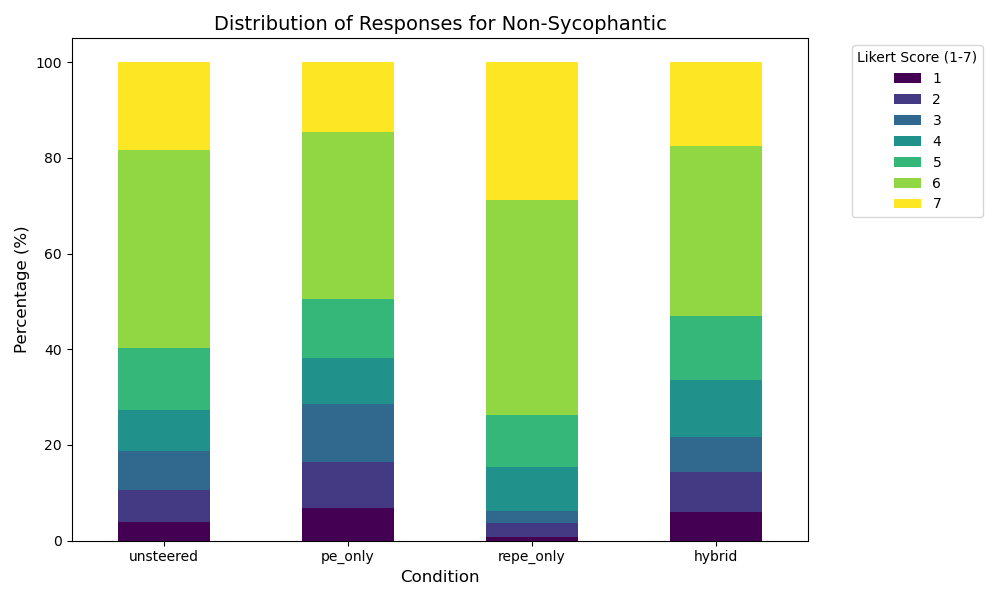
\includegraphics[width=0.9\columnwidth]{Figures/chart_Non-Sycophantic}
\caption{Distribution of non-sycophancy ratings (7-point Likert) across conditions. RepE-only steering produces the highest proportion of high non-sycophancy ratings (scores 6--7), confirming that representation-level steering effectively reduces sycophantic behaviour.}
\label{fig:charts}
\end{figure}

\subsubsection{Inter-Metric Correlations.}

Spearman correlations between the three metrics reveal: Appropriateness and Naturalness are strongly correlated ($\rho = 0.611$, $p < 10^{-275}$), while Non-Sycophancy shows moderate correlation with Naturalness ($\rho = 0.501$) and weaker correlation with Appropriateness ($\rho = 0.390$). This confirms that non-sycophancy is a partially independent quality dimension that is not fully captured by perceived appropriateness.

\section{Discussion}

\subsection{Complementary Strengths}

Our results reveal a clear complementarity between prompt engineering and representation steering. Prompt engineering excels at Evaluation steering, likely because specifying social roles (``Pretend you're a counselor'') alongside natural language instructions on how to behave in that role implicitly constrains the valence of responses. Representation steering excels at Potency and Activity, dimensions that are more closely tied to the \textit{how} of expression (assertiveness, energy level) rather than the \textit{what} (sentiment polarity). This distinction aligns with the linear representation hypothesis \citep{park2024linear}: style-level properties may be more linearly separable in hidden states than content-level properties.

\subsection{ACT as a Steering Target Source}

A key insight of this work is that sociological theory can provide principled steering targets for representation engineering. Prior work on RepE steering has focused on binary concepts (honest/dishonest, moral/immoral) with researcher-chosen coefficients. ACT provides three advantages: (1) continuous-valued targets calibrated to cultural norms, (2) situation-dependent targets that adapt to the specific social context, and (3) an explicit optimality criterion (deflection minimisation) grounded in decades of empirical sociological research.

\subsection{Sycophancy Reduction as an Emergent Property}

The sycophancy reduction we observe is not an explicit design goal but an \textit{emergent property} of ACT-aligned steering. ACT's deflection minimisation computes what a real person in the given social role would affectively do---not what would maximise the user's approval. For a \textit{counselor} responding to a \textit{client}'s praise, ACT predicts moderate warmth with professional authority---not effusive gratitude. By steering toward these sociologically grounded targets, the model naturally avoids the excessive agreeableness that characterises sycophancy.

\subsection{Comparison with Frontier Models}

Table~\ref{tab:steering} places our steered conditions alongside two frontier models queried through their public APIs. Because neither API exposes hidden states or a forward hook, only the unsteered and prompt-engineered conditions are available for them; representation steering is not possible at the API level. All conditions are scored by the same calibrated EPA reader, which operates on text alone and is independent of the model that produced it.

The hybrid condition on Llama-3.1-8B achieves the lowest overall distance (0.795), a 12.2\% reduction from the local unsteered baseline (0.905) and 16.0\% below the closest frontier configuration without an affective instruction (Gemini unsteered, 0.946). All three of our steered or prompted local conditions place ahead of every frontier configuration. The separation is driven almost entirely by Evaluation: local conditions fall between 0.645 and 0.759 on that dimension, while the frontier baselines range from 0.840 to 0.977. Potency shows no meaningful separation between any conditions, and Activity separates only weakly.

The frontier models therefore do not close the gap by scale alone. Adding an affective instruction to the prompt improves both of them (Claude 0.902 to 0.886; Gemini 0.946 to 0.893), but neither reaches the level of an 8B model steered toward ACT-derived targets at inference time. This supports the view that alignment to situation-specific affective targets is not an emergent property of capability, and that an explicit steering mechanism remains necessary.

\subsection{Limitations}

\textbf{Reading accuracy.} EPA reading achieves $\rho = 0.32\text{--}0.79$, introducing noise into the closed loop. Evaluation is read most reliably, while Activity lags behind. Improving Activity reading---potentially through better contrastive templates or multi-task training---would likely improve overall steering quality.

\textbf{Evaluation dimension.} RepE steering has negligible effect on Evaluation, the dimension most directly associated with sentiment. This may indicate that sentiment polarity is distributed across multiple representational subspaces that a single PCA direction cannot capture, or that the model's RLHF training creates strong resistance to evaluation shifts at the representation level.

\textbf{Human evaluation scale.} Our study uses 48 participants and 14 vignettes. While statistical power is adequate for the observed effect sizes ($H > 70$), a larger study with more diverse demographic representation would strengthen generalisability claims.

\textbf{Cultural specificity.} ACT dictionaries are culture-specific; our coefficients use the 2010 US interaction survey. Cross-cultural deployment would require corresponding sentiment dictionaries.

\section{Future Work}

The current system steers individual responses in isolation. Several natural extensions would bring it closer to a complete model of socially intelligent interaction.

\subsection{Multi-Turn Deflection Tracking}

The most immediate extension is to track ACT's deflection across an entire conversation rather than computing the optimal behaviour independently for each turn. In human interaction, transient impressions accumulate: a sequence of deflection-increasing behaviours produces compounding stress, while deflection-reducing behaviours gradually restore equilibrium. Implementing a \textbf{conversational deflection tracker} would maintain the running transient impressions across turns, feeding the post-event transients from turn $k$ as the pre-event fundamentals for turn $k+1$. This would enable the system to detect when a conversation is becoming increasingly strained (rising deflection) and respond with progressively stronger corrective steering, or to relax steering when the interaction is proceeding smoothly.

A key research question is how the reader's EPA noise ($\rho = 0.32\text{--}0.79$) accumulates across turns. Bayesian filtering over the EPA readings (see section below) could mitigate this by maintaining uncertainty estimates over the transient impressions.

\subsection{BayesACT Integration}

Bayesian Affect Control Theory (BayesACT; \citealt{hoey2013bayesact, schroeder2016modelling}) extends classical ACT by representing identities and sentiments as probability distributions rather than point estimates. This is particularly relevant for LLM steering because:

\begin{enumerate}
    \item \textbf{Uncertainty in EPA readings:} The reader produces noisy estimates ($\rho = 0.32\text{--}0.79$). BayesACT can propagate this uncertainty through the impression formation equations, yielding posterior distributions over optimal behaviour rather than point estimates. This would allow the system to adopt more conservative steering when EPA readings are uncertain.
    \item \textbf{Identity uncertainty:} In open-domain conversation, the user's social identity may not be known a priori. BayesACT maintains a distribution over possible identities and updates it as the conversation progresses, a form of \textit{identity inference}. This would enable the system to adapt its steering targets as it learns more about the user's social role.
    \item \textbf{Partially observable interactions:} BayesACT frames interaction as a Partially Observable Markov Decision Process (POMDP; \citep{hoey2016affect}), enabling principled planning over multi-turn trajectories. This would allow the system to reason about the long-term consequences of its affective choices, steering not just for the immediate turn but for the trajectory of the conversation.
\end{enumerate}

\subsection{Modifiers and Composite Identities}

Classical ACT supports \textbf{identity modifiers}---adjectives that shift the fundamental sentiments of an identity \citep{averett1987modified}. For example, an ``angry client'' has a different EPA profile from a ``grateful client,'' computed via empirically estimated amalgamation equations. Integrating modifier support would enable the system to handle more nuanced social scenarios where identities carry emotional or trait-based qualifications (e.g., ``anxious student,'' ``experienced doctor,'' ``frustrated customer'').

A related extension is support for \textbf{composite identities} where multiple role labels apply simultaneously (e.g., a user who is both a ``student'' and a ``friend''). ACT provides combination rules for these cases, but their integration with RepE steering---where the target EPA would change dynamically as the composite identity is inferred---remains unexplored.

\subsection{Reidentification}

When deflection remains persistently high despite optimal behaviour selection, ACT predicts that social actors engage in \textbf{reidentification}---reinterpreting the identity of one or more interactants to make the observed behaviour less surprising \citep{mackinnonheise2010self, heise2007expressive}. For example, if a ``friend'' consistently behaves in a hostile manner, ACT predicts that the other party will eventually reidentify them as an ``enemy'' or ``bully,'' fundamentally changing the affective dynamics of the interaction.

Implementing reidentification in the steering framework would require:
\begin{enumerate}
    \item \textbf{Deflection monitoring:} Tracking cumulative deflection across turns and triggering reidentification when it exceeds a threshold.
    \item \textbf{Identity search:} Searching the ACT dictionary for identities whose fundamental sentiments better explain the observed behaviour EPA pattern.
    \item \textbf{Dynamic target update:} Recalculating the optimal behaviour EPA under the new identity assignment and adjusting the steering targets accordingly.
\end{enumerate}

This would enable the system to handle adversarial or identity-shifting interactions gracefully, adapting its social model rather than persisting with a mismatched identity assignment.

\section{Conclusion}

We have presented a framework that bridges sociological theory and representation engineering to produce socially grounded LLM behaviour. Our approach computes situation-specific affective targets from ACT's deflection minimisation equations and steers generation via calibrated activation vectors, achieving significant improvements in affective alignment without weight modification. Human evaluation confirms that representation steering effectively reduces sycophancy---an emergent benefit of aligning to sociological norms rather than user preferences---while preserving naturalness. This work opens a new direction for inference-time behavioural control of LLMs, grounded in established social science rather than ad hoc engineering.

\section*{Ethical Statement}

This work uses ACT, which models culturally \textit{normative} (statistically average) affective expectations. These norms may encode societal biases present in the survey data (e.g., the 2010 US interaction survey). Deploying this system in practice requires careful consideration of whose norms are being enforced and whether they are appropriate for the target population. The system steers \textit{affective tone} without controlling \textit{content}, and should not be used as a sole mechanism for safety-critical applications without additional safeguards. All human evaluation data was collected anonymously with informed consent.

\bibliography{references}

\end{document}
